i%%%%%%%%%%%%%%%%%%%%%%%%%%%%%%%%%%%%%%%%%%%%%%%%%%%%%%%%%%%%%%%%%%%%%%%%%%%%%%%%

\documentclass[letterpaper,twocolumn,10pt]{article}
\usepackage{usenix2019_v3}

% to be able to draw some self-contained figs
\usepackage{tikz}
\usepackage{amsmath}
\usepackage{subcaption}

% inlined bib file
%\usepackage{filecontents}

%-------------------------------------------------------------------------------
\begin{document}
%-------------------------------------------------------------------------------

%don't want date printed
\date{}

%maketitle
% make title bold and 14 pt font (Latex default is non-bold, 16 pt)

\title{Impact of OS Design and Hardware Configuration on the Power Performance Tradeoff}

%  An (Incomplete) Example}

%for single author (just remove % characters)
%\author{
%{\rm Your N.\ Here}\\
%Your Institution
%\and
%{\rm Second Name}\\
%Second Institution
% copy the following lines to add more authors
% \and
% {\rm Name}\\
%Name Institution
%} % end author

 \maketitle


\begin{abstract}
Energy proportional computing is a challenging feat when faced with the management of modern I/O intensive datacenter workloads with strict service level agreements (SLAs). We focus on saving power in the context of key-value stores that have 99\% tail latencies in the hundreds of microseconds. Typically, additional power savings can be gained when server nodes are underutilized during periods of low to medium traffic by using CPU power limiting or frequency tuning methods. In this work, we tackle power consumption in relation to the dual operation of system software stacks and network interface cards (NICs). We first explore manipulating a time-based interrupt throttling mechanism on modern NICs to tune interrupt rates and control the batching of packet processing. By exploiting this feature and artificially increasing packet processing delay, a system is able to buffer more packets and process less interrupts. This method was able to achieve over 22\% power savings  compared to using CPU power limiting features when used in Linux. 

  We also compare and contrasted CPU and NIC tuning in the context of a baremetal library OS specialized for Memcached in order to understand their behavior in the performance-power tradeoff. Our baremetal library OS was able to achieve 2.5X higher peak throughput than Linux while using 3X lower power. Moreover, we find that our library OS is more than 2-3X more efficient in number of instructions per watt used, and therefor is more sensitive to CPU frequency changes. Our results demonstrate that optimizing the dataplane code path in system software stacks paired with the right hardware tuning can scale up I/O intensive workloads while effectively lowering power consumption.
\end{abstract}


%-------------------------------------------------------------------------------
\section{Introduction}
%-------------------------------------------------------------------------------
There is a fundamental tension between performance guarantees and energy consumption in modern datacenter workloads. They are often single purpose~\cite{workloadanalysisfacebook, WebSearch, svefacebook, profilewhscomputer} and I/O intensive with strict service level agreements (SLA) ranging from hundreds of microseconds to milliseconds~\cite{tailatscale, scalingmcdfacebook}. Kernel bypass~\cite{ix, farm, dpdk, arrakis}, and kernel specialization~\cite{rumpkernel, unikernels, ebbrt} methods have been proposed to address the performance problems. However, datacenters are already under increasingly constrained energy budgets~\cite{SmoothOperator, Dynamo}. This complicates achieving their performance targets and puts pressure on general purpose system software stacks to be efficient in order to provide the throughput and latency guarantees.

The class of online, data-intensive (OLDI) workloads, one of which is Memcached~\cite{memcached}, have been well studied from this perspective~\cite{10.1145/2678373.2665718, 10.1145/2806777.2806848, 10.1145/2024723.2000103, napsac}. Memcached workloads typically have a high fan-out deployment on many user facing servers with stringent SLAs in hundreds of microseconds. The Memcached service must also sustain high request rates and many incoming connections while maintaining the SLA specified low tail latencies. In addition, these workloads can operate in low to medium utilization levels due to diurnal patterns in user traffic~\cite{workloadanalysisfacebook, 10.1145/2024723.2000103}. One way to improve energy efficiency of OLDI workloads under stringent SLAs is to scale a node's power consumption down under low to medium utilizations while satisfying the current SLA. Prior works~\cite{10.1145/2678373.2665718, 10.1145/2806777.2806848} have tackled this specific problem by using features on modern processors to modulate power consumption of CPUs, namely Running Average Power Limit (RAPL)~\cite{intel_rapl} and Dynamic Voltage Frequency Scaling (DVFS) ~\cite{cpufreq_governor}.

\begin{figure}
  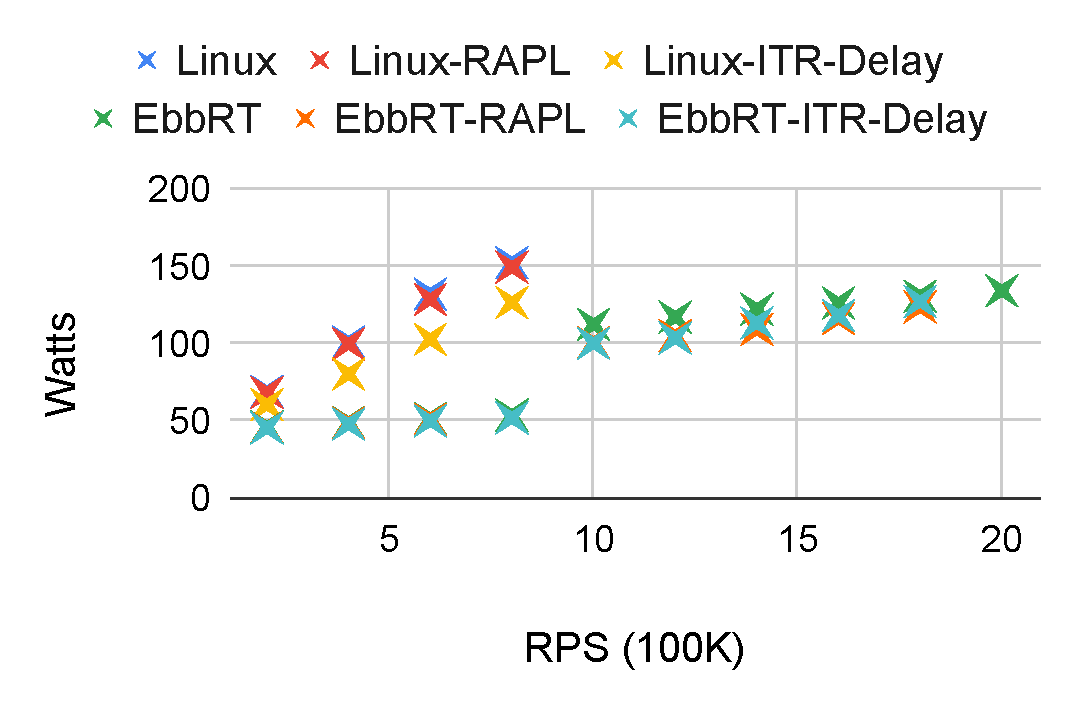
\includegraphics[width=7.9cm]{chart.pdf}
  \caption{Performance vs Watts used}
  \label{fig:chart}
\end{figure}

While the approach of exploiting hardware mechanisms to provide just enough performance to meet the required SLA is compelling, is limiting the power or frequency of the processor the most effective technique for I/O intesive workloads?  We hypothesize that a hardware mechanism that directly correlated to the delay of requests could be more effective.  To test this hypothesis, we explore using a hardware feature available on most modern network interface cards (NICs) that limit maximum interrupt rates. The Intel 82599 datasheet~\cite{82599} defines a time-based interrupt throttling mechanism to limit maximum interrupt rates. We refer to this as \textit{ITR-Delay}, it controls the time delay between packet reception and firing of the interrupt on a particular core. The effect of setting a higher interrupt delay can cause more receive packets to be buffered and increase packet processing efficiency at a potential cost to response time. By default, the IXGBE device driver~\cite{intel_ixgbe} updates the interrupt delay value dynamically after every packet receive to the interrupt delay value such that it can better handle the current traffic pattern. This value can also be tuned statically, which results in a interrupts being fired statically every X microseconds, where X is a configurable value. We take advantage of this ability by setting interrupt delay values statically for different request loads while maintaining SLA tail latency objectives. We find that controlling the batching of packet processing that happens underneath a complex system software stack can help find a sweet spot in performance to energy consumption ratios. Under a general purpose OS, we demonstrate a reduction in energy consumption by up to 22\% compared to using \textit{RAPL} power limiting in running Memcached.

Furthermore, there has been a lot of renewed interest in different specialized software stacks such as Unikernels and Library OSes to satisfy demand of modern datacenter workloads~\cite{unikernels, aliraza}. They have shown benefits by optimizing the dataplane code path in order to scale up workloads such as Memcached. To understand how the unikernel approach compares to our hardware based one, we ported an existing library OS, EbbRT~\cite{ebbrt}, that was developed for virtualized environments, to run on bare metal directly using the same physical NIC. While EbbRT virtualized was able to achieve 1.5X higher peak throughput than Linux native, Figure~\ref{fig:chart} shows that baremetal EbbRT was able to achieve more than 2.5X higher peak throughput.

We also explored the effects of tuning the same set of hardware knobs (\textit{ITR-Delay}, \textit{RAPL}, and \textit{DVFS}) in the context of a baremetal library OS for Memcached. The goal is to understand the performance and power implications when an entire systems software stack is different. Figure~\ref{fig:chart} shows that by applying power limiting features and interrupt delay mechanisms, we are able to achieve an additional 16\% in power savings when the CPU frequency is set at the highest frequency. It also shows that baremetal EbbRT is able to sustain the same request loads of running Memcached in Linux by using up to 3X less power when CPU frequency is set at the lowest frequency. This is partly due to the fact that EbbRT uses up to 3X fewer instructions than Linux to handle the same SLA objective in a multi-core Memcached experiment. 

In the rest of the paper, we first explain the interrupt delay mechanism on the NIC and how it interacts with a general purpose OS stack such as Linux. We also shown how its dynamic interrupt delay is functioning during a Memcached workload. Next, we go into detail about how we set up the hardware, in terms of CPU configurations via the Intel Model Specific Registers (MSRs), how it is replicated in EbbRT and the multi-node experimental setup. We then describe two simple methods, \textit{RAPL-MIN} and \textit{ITR-MAX}, which are two iterative methods at finding peak power limit and maximum interrupt delay limit such that they maximize power while ensuring 99\% tail latencies are still under the SLA objective. Finally, we present our experimental results in Section~\ref{sec:res}. We also discuss future directions.

\section{Network Device Drivers}
\begin{figure}
  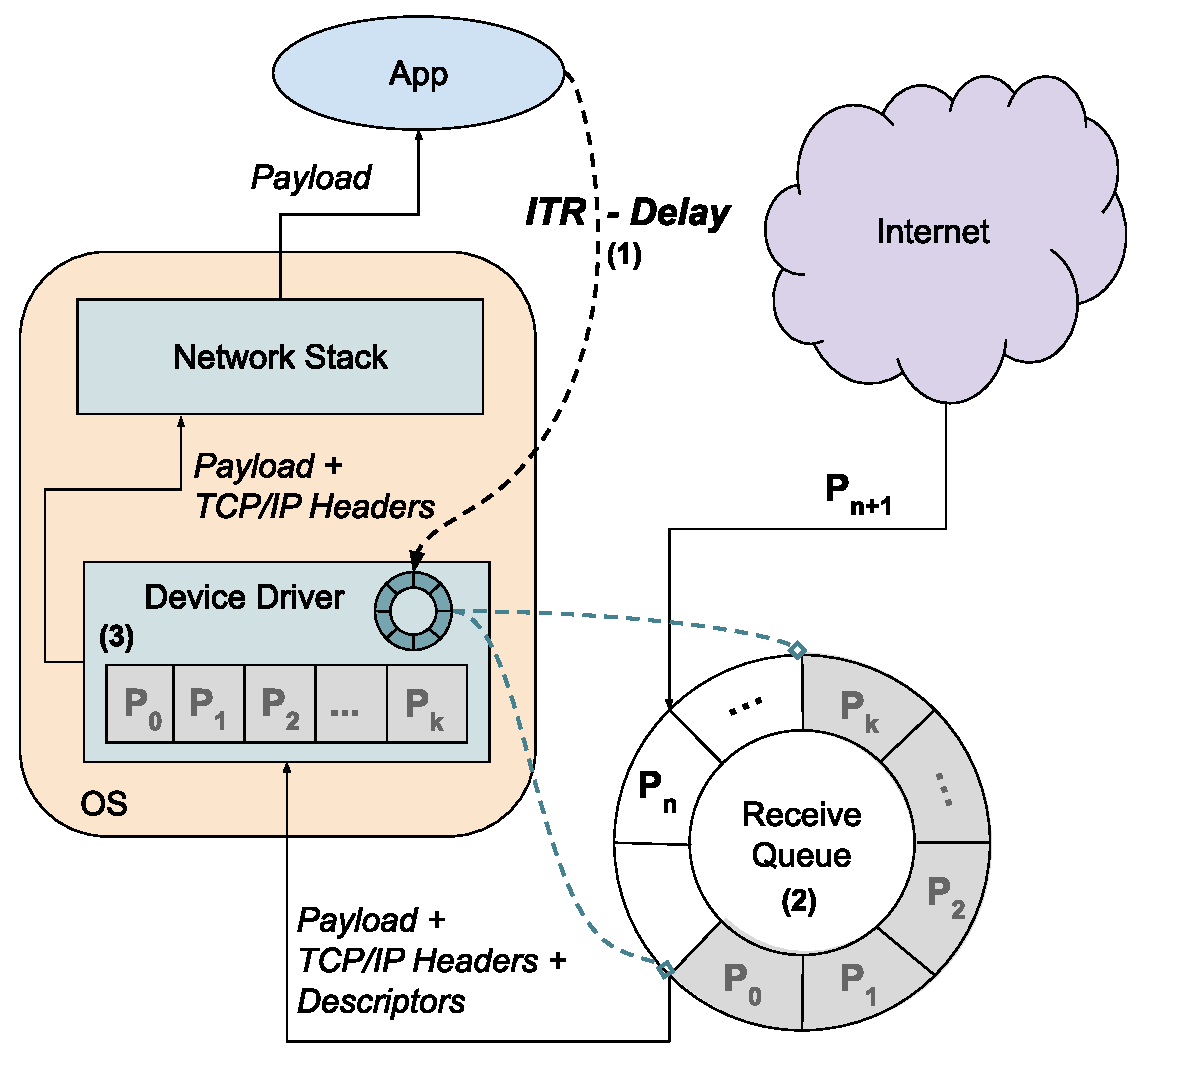
\includegraphics[width=7.7cm]{itr_figure.pdf}
  \caption{\textit{ITR-Delay} mechanism.}
  \label{fig:itr_figure}
\end{figure}

In this work, we use the Intel 82599ES 10GbE NIC in our experiments for \textit{ITR-Delay} tuning. Figure~\ref{fig:itr_figure} illustrates this mechanism of \textit{ITR-Delay} in the context of a general system. \textit{ITR-Delay} is a hardware knob that is exposed as a set of bits within a hardware register in the Intel 82599 datasheet~\cite{82599}. In Linux, this hardware knob can be accessed via the \textit{rx\_usecs} parameter in \textit{ethtool}. This parameter is tuned soley within the IXGBE device driver via a policy to improve the performance of packet processing. Figure~\ref{fig:itr_figure} shows the overall process of how interrupt delays impact packet processing.
As \textit{ITR-Delay} (1) is turned up, this causes the NIC's Receive Queue (2) to buffer more incoming packets as the NIC cannot fire new interrupts until the delay value has been reached.
Once the interrupt is fired, Linux's NAPI polling mechanism kicks in and starts polling in new packets (3) to be processed until it either reaches its current work budget or if there is no more data to be processed. The 82599 NIC enables us to set interrupt delay values at a granularity of 2 microseconds and it can range from 0 to 1024 microseconds, where 0 indicates that an interrupt is fired for every packet receive, while 1024 means the device will wait for 1024 microseconds before initiating the next interrupt.
%Another part of our motivation in tuning this parameter is understanding whether hardware tuning matters given the complexity of other policies in Linux such as scheduling, and NAPI polling. We treated all software above the IXGBE device driver as a black box in order to gain better understanding of the impacts of changing hardware parameters, whether in Linux or a specialized kernel.

\begin{figure}
  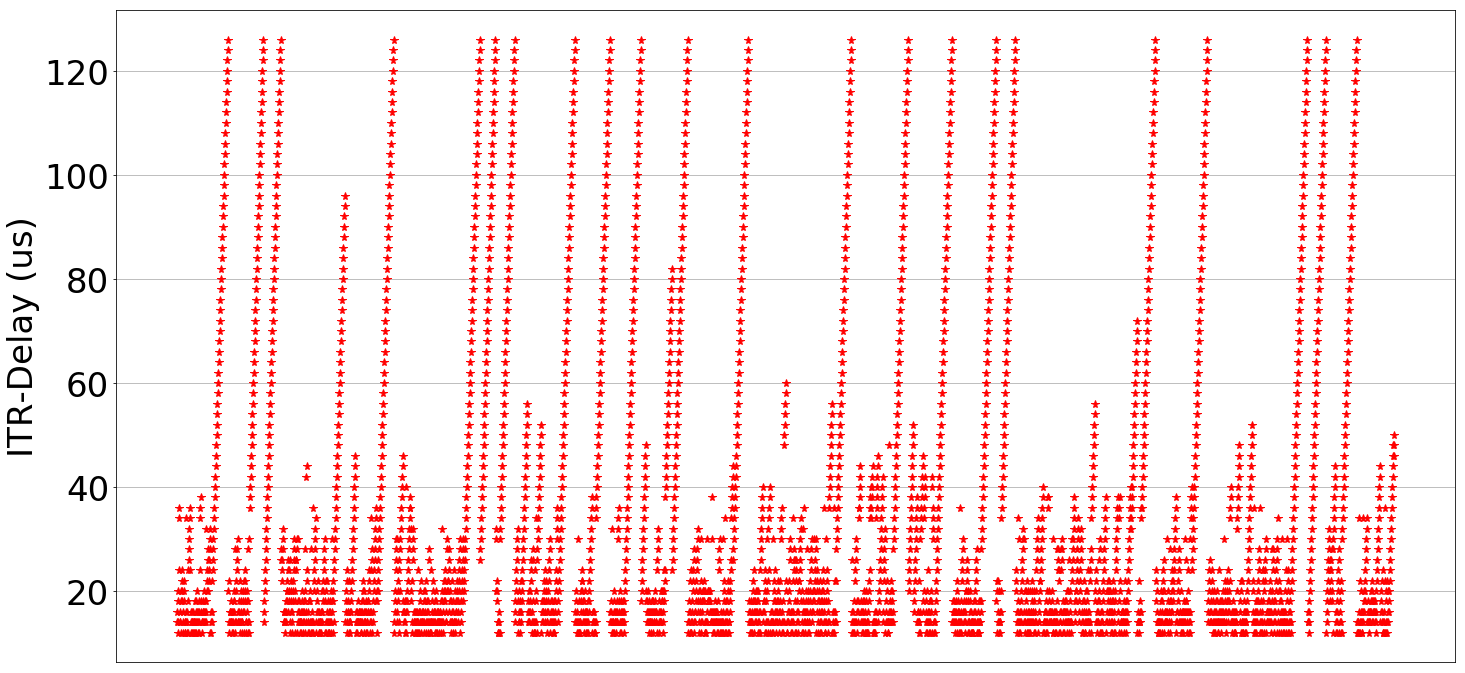
\includegraphics[width=8cm]{itr_delays.png}
  \caption{Updated interrupt delay values during memcached.}
  \label{fig:itr_delays}
\end{figure}

In Linux's IXGBE device driver, there is a dynamic algorithm that seeks to tune \textit{ITR-Delay} such that it better reflects the current workload.
It achieves this by using packets and bytes received from the last interrupt and classifies them broadly into a set of ranges that are pre-computed based off theoretical maximum wire speeds.
Based off these ranges, they are then \texttt{switched} to a new delay value for the next interrupt.
To demonstrate its behavior, we instrumented a simple logging tool into the IXGBE device driver.
Figure~\ref{fig:itr_delays} shows a small snapshot of its values while running a Memcached workload.
Each marker represents a new \textit{ITR-Delay} value.
In its current implementation, it can only seek values between the range of 2 to 126 microseconds.
The reason for this is that it was never designed towards a use case of aggressively delaying packet receive interrupts to take advantage of energy proportionality under stringent SLAs, which can potentially result in setting \textit{ITR-Delay} values in the hundreds of microseconds.

It is also possible to disable this dynamic algorithm through the flip of a bit inside the device driver.
This requires a rebuild of the driver module as it was not a configurable parameter.
After flipping this bit, we can use Linux's \textit{ethtool} to set new interrupt delay values statically to fire every X microseconds, where X is a configurable value.
In our experimentation, we take advantage of this ability by setting interrupt delay values statically for different request loads while maintaining SLA tail latency objectives.

EbbRT's IXGBE device driver is written in C++ and totals over 3000 lines of code.
It interfaces with a multicore TCP/IP network stack.
We were careful to ensure that both EbbRT and Linux were configured similarly in terms of NIC features: receive-side coalescing (RSC) disabled, direct-cache injection (DCA) disabled, receive-side scaling (RSS) enabled to distribute packets for multi-core processing, hardware checksum offloading enabled.
We also ensured the same values for parameters such as number of NIC transmit, receive descriptors and write-back thresholds for packet transmissions.
A main difference in EbbRT is that it inherently does not have a dynamic policy for updating interrupt delay values since its implementation in Linux relies on other assumptions such as jiffies and NAPI polling budgets.
%In our comparison results below, we seek to approximate this dynamic algorithm by using a static interrupt value that mirrors its performance and power.

\section{System Configuration}
In our experiments, we use static configurations of \textit{DVFS}, \textit{RAPL}, and \textit{ITR-Delay} in the following ways:
\begin{itemize}
\item Initially, \textit{DVFS} is used to configure both Linux and EbbRT to the same CPU frequency.
Linux is configured by overwriting each CPU's \textit{cpufreq/scaling\_governor} into various states.
We explored two frequency states: \textit{performance} and \textit{powersave}, which represent the lowest and highest frequency avaiable on the processor.
The main reason was to highlight the extremities in configuration to better understand differences when we apply additional power limiting and interrupt delay mechanisms.
We validated that the above methods are correct in that new updated values appear in both IA32\_PERF\_CTL and MSR\_PERF\_STATUS registers~\cite{intel_msr}.
In EbbRT, the same updated values are written to the corresponding MSRs to toggle between low and high CPU frequencies.
\item \textit{ITR-Delay} exists in two modes, the first is with the default policy that dynamically updates its value per receive interrupt (\textit{ITR-DYNAMIC}), while the second is a static interrupt value.
In Linux, both modes are explored in conjunction with the aforementioned \textit{DVFS} states.
In the static mode, a simple method of exploration is to repeatedly rerun the same workload but incrementally increase the interrupt delay value such that for a particular request load, the tail latencies lie just under the SLA.
We indicate this as ~\textit{ITR-MAX} in our results section.
\item \textit{RAPL} is applied in Linux in conjunction with \textit{DVFS} states using the same approach as \textit{ITR-MAX} but by iteratively decreasing the CPU's power limit until either the SLA objective is violated, the Memcached process fails to launch, or Memcached fails to create the necessary number of connections. The method used is indicated as ~\textit{RAPL-MIN} in the results below.
We did not explore \textit{RAPL} and \textit{ITR-Delay} together as the search space would have been too large.
\end{itemize}

\begin{figure}
  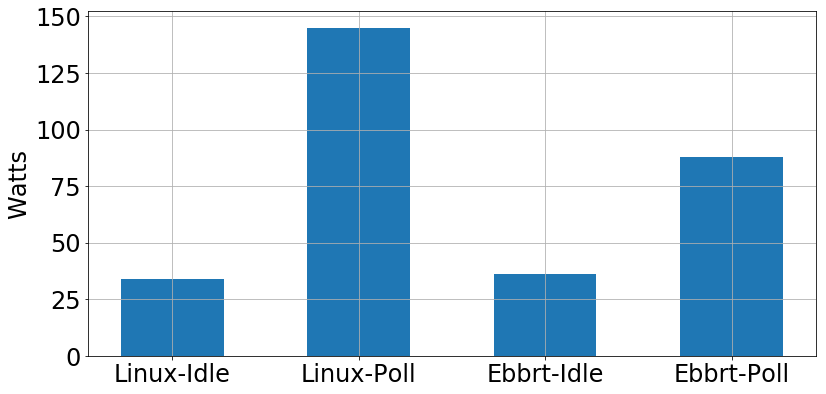
\includegraphics[width=8cm]{ebbrt_linux_poll_compare.png}
  \caption{Power usage in poll and idle modes.}
  \label{fig:ebbrt_linux_poll}  
\end{figure}

In addition, we ensured that the processor for both Linux and baremetal EbbRT was setup as similarly as possible by carefully configuring both IA-32 Architectural MSRs (Table 35-2) and processor specific MSRs (Table-35-18) in Intel's system programmer's manual~\cite{intel_msr}. One of EbbRT's design point is an event-driven model, its event loop is designed such that an interrupt that is continously fired after every static period of time has passed. To implement a similar CPU idle function as Linux, we added a MONITOR and MWAIT instruction in the event loop code to force it always to go into the C7 sleep state prior to an execution of a HLT instruction. Given this, Figure~\ref{fig:ebbrt_linux_poll} illustrates the base efficiency of a specialized kernel. We use the Intel \textit{RAPL} provided MSR\_PKG\_ENERGY\_STATUS register was used to gather CPU power usage numbers. In polling mode, EbbRT results in a power savings of 39\% over Linux.
\begin{figure}
 \begin{subfigure}{0.5\textwidth}
   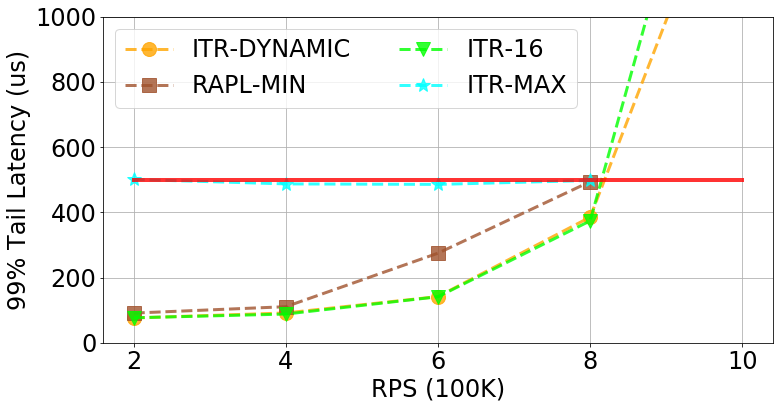
\includegraphics[width=\textwidth]{linux_etc_perf_sla.png}
   \caption{}
   \label{fig:linux_etc_perf:sla}
 \end{subfigure}
  \begin{subfigure}{0.5\textwidth}
   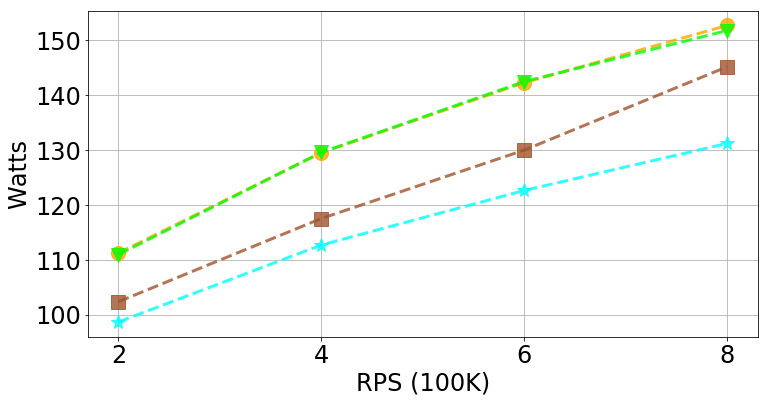
\includegraphics[width=\textwidth]{linux_etc_perf_watts.png}
   \caption{}
   \label{fig:linux_etc_perf:watts}
  \end{subfigure}
  \begin{subfigure}{0.5\textwidth}
   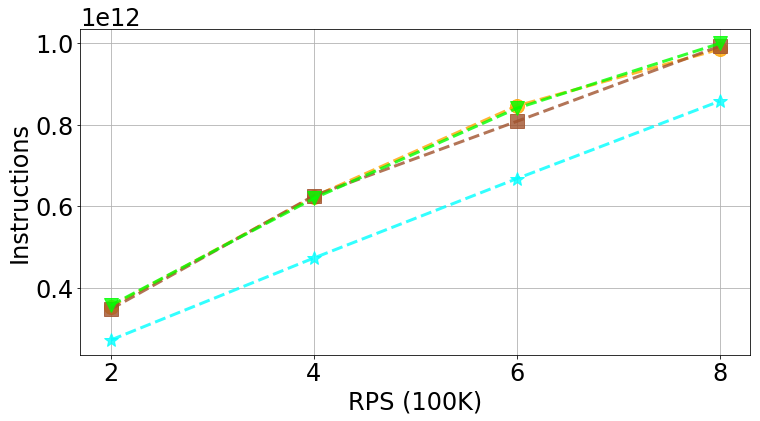
\includegraphics[width=\textwidth]{linux_etc_perf_ins.png}
   \caption{}
   \label{fig:linux_etc_perf:ins}
  \end{subfigure}
  \begin{subfigure}{0.5\textwidth}
   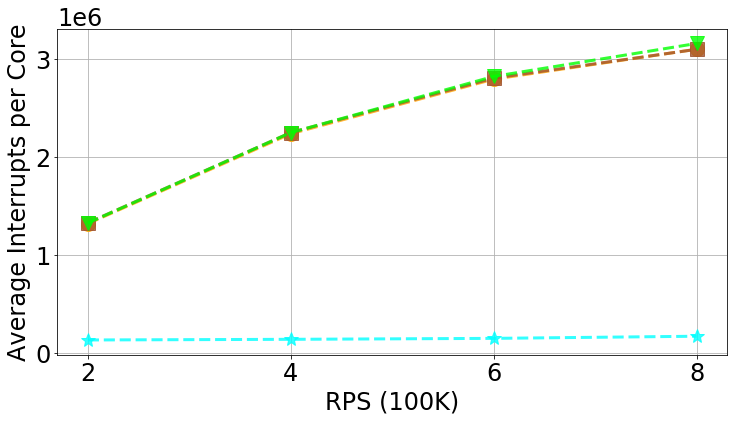
\includegraphics[width=\textwidth]{linux_etc_perf_itr.png}
   \caption{}
   \label{fig:linux_etc_perf:itr}
  \end{subfigure}
  \caption{Linux Memcached ETC workload in \textit{maximum} CPU frequency.}
  \label{fig:linux_etc_perf:main}
\end{figure}

\section{Experimental Approach}
\label{sec:exp_app}
Our experimental cluster consists of a total of 7 nodes with a mix of 16 core Intel(R) Xeon(R) CPU E5-2690 @ 2.90GHz and 12 core Intel(R) Xeon(R) CPU E5-2630L v2 @ 2.40GHz processors and NICs with a mix of Solarflare Communications SFC9120 10G Ethernet Controller, and Intel Corporation 82599ES 10-Gigabit SFI/SFP+. All the processors have hyperthreads and Turbo Boost feature disabled. All workloads are pinned to physical cores to reduce potential background noise. In addition, ~\textit{irqbalance} is disabled and packet receive interrupts are affinitized to their respective cores. The nodes have a mix of 125 GB RAM and 251 GB RAM configurations. We run memcached-1.5.6 on top of a Ubuntu LTS 18.0.4 installation with Linux 4.15.1, the other nodes either run Ubuntu LTS 18.0.4 with a mix of Linux 4.15.1 and 5.0.0 or Red Hat Enterprise Linux 7.7 with Linux 3.10.0.

The same server node is also used to boot into baremetal EbbRT. It contains a 16 core Intel(R) Xeon(R) CPU E5-2690 @ 2.90GHz, with 125 GB of RAM and a Intel Corporation 82599ES 10-Gigabit SFI/SFP+ NIC. In contrast to Linux, EbbRT uses a re-implemented version of memcached written to EbbRT interfaces. It is a multicore application that supports the standard memcached binary protocol. To alleviate lock contention, a RCU hashtable is used to store key-value pairs. EbbRT's implementation does lack some additional features such as authentication and other commands but it is functional enough to support the benchmark tool. 

We run Memcached on all 16 cores on the server node, the SLA objective in our experiments is to maintain tail latency of 99\% requests under 500 us. There is another unloaded client node running \textit{mutilate} as the master node for controlling and monitoring the experiment, it has two responsibilities: 1) coordinates with five other ~\textit{mutilate} slave nodes to generate requests to the Memcached server and, 2) it measures tail latencies of all requests made. Two of the five nodes are 12 core machines while the rest are all 16 core machines. Each core creates 16 connections, for a total of 1152 connections amongst 5 nodes for a single memcached server. This setup is able to saturate the single 16 core server. We configured ~\textit{mutilate} to pipeline up to four connections to further increase its request rate. We run a representative load from Facebook~\cite{workloadanalysisfacebook} (ETC), which represents the highest capacity deployment, it uses 20 Byte - 70 Byte keys, and 1 Byte to 1 KByte values, and contains 75\% GET requests.

Given a static configuration listed above, we use \textit{mutilate} to generate loads at different request per second (RPS) rates, each for a constant period of time while collecting additional system metrics. In Linux, \textit{perf} is used to gather these metrics at a per second timeslice since the MSR\_PKG\_ENERGY\_STATUS for reporting CPU power usage has a limited wrap around time. EbbRT is able to collect the same metrics as Linux as it contains a inbuilt ~\textit{Perf} class which reads directly from Intel's PMC registers and a ~\textit{Rapl} class which reads from Intel's RAPL registers. In EbbRT, an event is triggered to fire every second in order to log the corresponding data.
\begin{figure}
 \begin{subfigure}[b]{0.48\textwidth}
   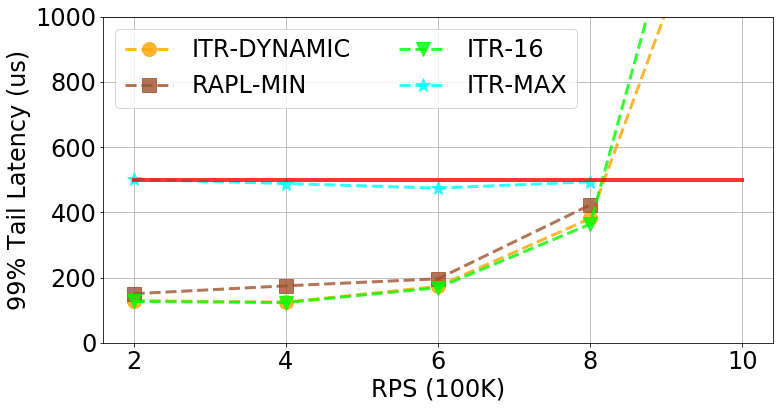
\includegraphics[width=\textwidth]{linux_etc_pow_sla.png}
   \caption{}
   \label{fig:linux_etc_pow:sla}
    \end{subfigure}

\begin{subfigure}[b]{0.48\textwidth}
   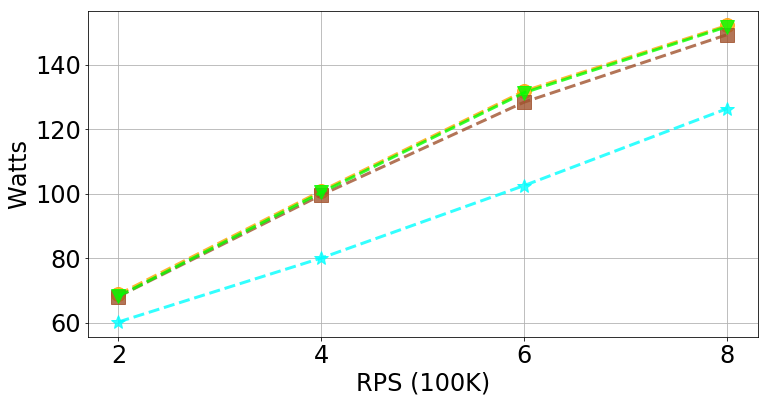
\includegraphics[width=\textwidth]{linux_etc_pow_watts.png}
   \caption{}
   \label{fig:linux_etc_pow:watts}
  \end{subfigure}
  \caption{Linux Memcached ETC workload in \textit{minimum} CPU frequency.}
  \label{fig:linux_etc_pow:main}
\end{figure}

\section{Results}
\label{sec:res}
\subsection{Linux}
In this section, we examine the power savings achievable in Linux when running Memcached at different RPS loads. Two methods are used, namely \textit{RAPL-MIN} and \textit{ITR-MAX} and the CPU frequency is at the highest. We also captured other metrics such as number of instructions and number of interrupts fired per core during each experiment to better understand efficiency gains. Figure~\ref{fig:linux_etc_perf:sla} illustrates the 99\% tail latency as a function of different request loads for Linux when configured with maximum CPU frequency. \textit{ITR-MAX} is able to maximize SLA gap to drastically increase tail latency of requests such that they are consistently shifted just under the SLA objective, as indicated by the red line. In contrast, power limiting in \textit{RAPL-MIN} is not able to achieve the same level of precision across the various request loads compared tuning NIC hardware registers. One reason is that \textit{RAPL} power limiting is applied across the entire CPU die, which is a coarser-grained method that impacts all system components, therefore it is difficult to fully exploit the opportunity gaps during low to medium utilization of request loads while meeting SLA objectives. By aggressively delaying packet receive interrupts, \textit{ITR-MAX} can enable more efficient packet processing by interacting with the NAPI polling algorithm in the IXGBE device driver. After every receive interrupt, NAPI polling will poll the receive descriptors for a period of time to process as many packets as it can within its given budget. This results in better coalescing of incoming packets and fewer wasted instructions on handling interrupts and other system work that needs to be done to handle every interrupt received. The immediate effect of this can be seen in Figure~\ref{fig:linux_etc_perf:itr} where \textit{ITR-MAX} uses more than 10X fewer interrupts per core to satisfy the same request load. With fewer interrupts to process, \textit{ITR-MAX} also uses between 14\%-22\% fewer instructions as shown in Figure~\ref{fig:linux_etc_perf:ins}. Compared to the power usage of default Linux (\textit{ITR-DYNAMIC}), Figure~\ref{fig:linux_etc_perf:watts} shows \textit{RAPL-MIN} was able to achieve power savings between 5\%-9\% whereas \textit{ITR-MAX} was able to achieve power savings between 11\%-14\%.

As an aside, we found a static interrupt delay of 16 microseconds (~\textit{ITR-16}) was able to approximate the same performance and power used as \textit{ITR-DYNAMIC}, it is also prominently featured in the denser regions of Figure~\ref{fig:itr_delays} under 20 microseconds. We wanted to highlight this in our graphs as it shows that the current dynamic policy in the IXGBE device driver is not necessarily targetted towards the benefit of an application such as Memcached, when one wants to delay packet processing until tail latencies are just barely meeting SLA objectives. In contrast, what we've shown is that by catering the policy in a way such that it aggressively increases interrupt delay values while still being able to maintain the same request load under the SLA, we are able to do a more precise job in tackling this performance and power tradeoff.

The same experiment as above is conducted with the CPU frequency is set at the lowest in Figure~\ref{fig:linux_etc_pow:main}. We can see that the peak performance of Memcached has not changed much compared to running at maximum frequency. To examine whether there is a real difference between maximum and minimum peak performance, we conducted further tests by slowly increasing RPS at smaller granularities and found that maximum frequency was only able to reach a higher peak throughput of 0.1\% over the processor set at minimum frequency. This result suggests that Linux contains other system overheads that impede its ability to take advantage of the higher clock frequency to improve peak performance. In terms of comparing relative performance levels, the peak power savings using \textit{ITR-MAX} in Figure~\ref{fig:linux_etc_perf:watts} and Figure~\ref{fig:linux_etc_pow:watts}, Memcached is able to maintain the same request loads while using 4\%-40\% less power at lowest CPU frequency. However, using \textit{RAPL-MIN} in this setting had a minimal effect on power savings. At a RPS of 600K, Figure~\ref{fig:linux_etc_pow:watts} shows \textit{RAPL-MIN} managed an additional power savings of only 2.5\% with whereas using \textit{ITR-MAX} we were able to achieve 22.2\% additional power savings. \textit{RAPL} power limiting functions by setting a specific power limit during some average period of time that the processor can draw, therefore throttling its performance. This power limit is typically the Thermal Design Power (TDP) set by the manufacturer. This result suggests that when the processor is already running at minimum frequency (drawing the least amount of power), \textit{RAPL} is not as effective a method to save additional power.

%

\subsection{EbbRT}
\subsubsection{Maximum Processor Frequency}
\label{sec:ebbrt_max}
\begin{figure}
 \begin{subfigure}[b]{0.5\textwidth}
   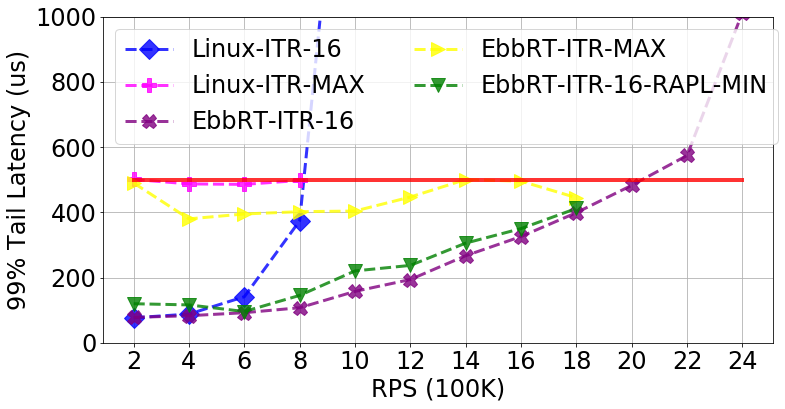
\includegraphics[width=\textwidth]{ebbrt_etc_perf_sla.png}
   \caption{}
   \label{fig:ebbrt_etc_perf:sla}
 \end{subfigure}
 \begin{subfigure}[b]{0.5\textwidth}
   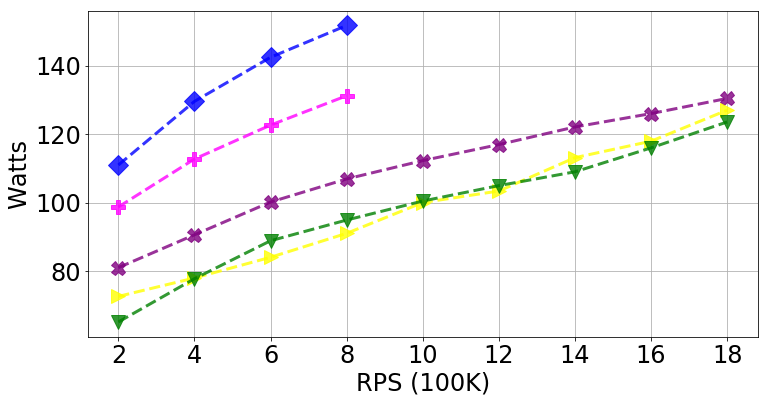
\includegraphics[width=\textwidth]{ebbrt_etc_perf_watts.png}
   \caption{}
   \label{fig:ebbrt_etc_perf:watts}
 \end{subfigure}
 \begin{subfigure}[b]{0.5\textwidth}
    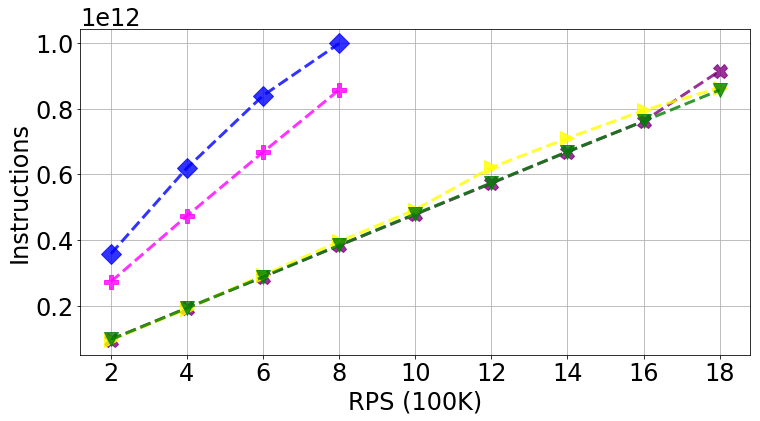
\includegraphics[width=\textwidth]{ebbrt_etc_perf_ins.png}
    \label{fig:ebbrt_etc_perf:ins}
  \end{subfigure}
  \begin{subfigure}[b]{0.5\textwidth}
    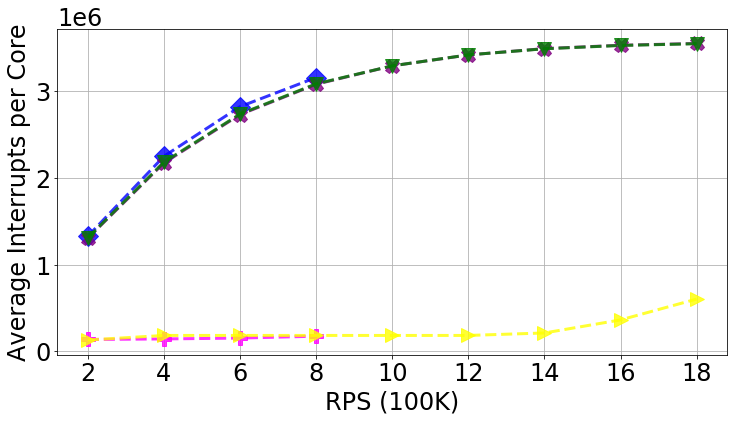
\includegraphics[width=\textwidth]{ebbrt_etc_perf_itr.png}
    \label{fig:ebbrt_etc_perf:itrs}
  \end{subfigure}  
  \caption{EbbRT Memcached ETC workload in \textit{maximum} CPU frequency.}
  \label{fig:ebbrt_etc_perf:main}
\end{figure}

\begin{table}[h!]
\centering
\begin{tabular}{ |c|c|c|c|c| } 
 \hline
 RPS(100K) & 2 & 4 & 6 & 8 \\
 \hline
 Linux-ITR-16 & 3.2e+09 & 4.8e+09 & 5.9e+09 & 6.6e+09 \\
 EbbRT-ITR-16 & 1.2e+09 & 2.1e+09 & 2.9e+09 & 3.6e+09 \\
 %Linux-ITR-MAX & 2.7e+09 & 4.2e+09 & 5.4e+09 & 6.5e+09 \\
 %EbbRT-ITR-MAX & 1.3e+09 & 2.4e+09 & 3.5e+09 & 4.3e+09 \\
 \hline
\end{tabular}
\caption{Instructions/Watt comparison at different request loads for static interrupt delay at 16 microseconds.}
\label{tab:ins_per_watt}
\end{table}

There have been plenty of works in the past that seek to improve Memcached performance in Linux through systems software specialization methods~\cite{mica, ebbrt, ix, mctp, arrakis}. While they seek the peak performance that could be gained, we are also curious about their implications in power usage and the tension in the power-performance tradeoff. Figure~\ref{fig:ebbrt_etc_perf:main} compares a baremetal library OS, EbbRT, with Linux when the processor is set at highest frequency. Given that EbbRT does not have a dynamic way of setting interrupt delay values, we used a static interrupt delay of 16 microseconds (ITR-16) as a representative comparison point against Linux. Memcached written to EbbRT's interfaces was able to achieve 2.5X higher peak throughput compared to Linux. The benefits of EbbRT's implementation was demonstrated previously in a virtualized environment and achieved 1.5X higher throughput running in a VM versus baremetal Linux~\cite{ebbrt}. Therefore, running baremetal EbbRT enabled us to achieve even further performance as we bypass additional system overheads inside the VM. Being a specialized unikernel for Memcached, it also uses 2.1X-2.8X fewer instructions to support the request rate in Linux. In contrast to the NAPI polling policy, EbbRT is not limited by a polling budget per receive interrupt, it will process as many receive descriptors as the hardware allows in a synchronous manner, moreover as interrupts are disabled during this entire process, EbbRT potentially could process more packets than Linux which must balance workload with processing budgets. This point is reflected in the amount of interrupts fired per core where on average EbbRT \textit{ITR-16} used 3\% fewer interrupts per core compared to Linux. From a efficiency perspective, Figure~\ref{fig:ebbrt_etc_perf:watts} shows EbbRT was able to satisfy the same request load as Linux but use 30\% less power on average.

We are also interested in comparing and contrasting the effects of tuning the same set of hardware knobs (\textit{ITR-Delay}, \textit{RAPL}, and \textit{DVFS}) in the context of a baremetal library OS for Memcached. Figure~\ref{fig:ebbrt_etc_perf:watts} shows the power savings achieved in EbbRT by using \textit{ITR-MAX}, similarly to Linux under maximum processor frequency~\ref{fig:linux_etc_perf:watts}, \textit{ITR-MAX} was able to further increase power savings compared to \textit{EbbRT-ITR-16} from 3\% to 17\%. In contrast to Linux, using \textit{RAPL-MIN} in EbbRT was able to achieve similar power savings as using \textit{ITR-MAX}, we believe this is partly due to the prototype implementation of the IXGBE device driver in EbbRT as it is not fully optimized yet, further, Table~\ref{tab:ins_per_watt} indicates that EbbRT uses less than of the Instructions per Watt at supporting the same workload as Linux, therefore power limiting has more of an impact as compared to Linux because EbbRT instructions are used more directly in executing the Memcached workload. Table~\ref{tab:ins_per_watt} also helps explain why at peak throughput of 1800K RPS, EbbRT is able to achieve 2.25X higher throughput while using similar power as Linux did at peak throughput of 800K.

\subsubsection{Minimum Processor Frequency}
\begin{figure}
  \begin{subfigure}[b]{0.5\textwidth}
    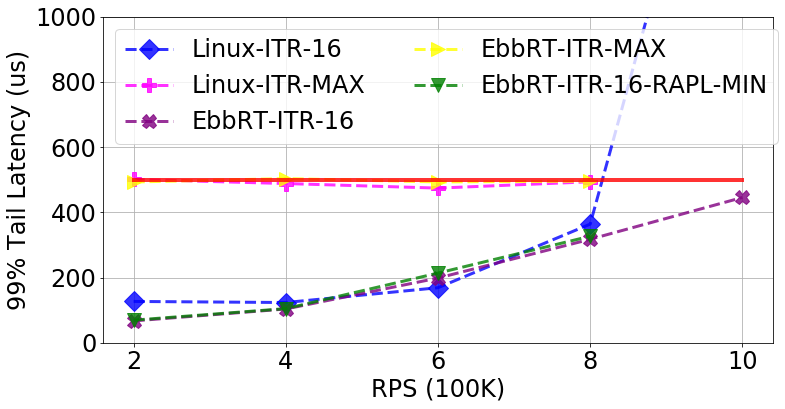
\includegraphics[width=\textwidth]{ebbrt_etc_pow_sla.png}
    \caption{}
    \label{fig:ebbrt_etc_pow:sla}
  \end{subfigure}
  \begin{subfigure}[b]{0.5\textwidth}
    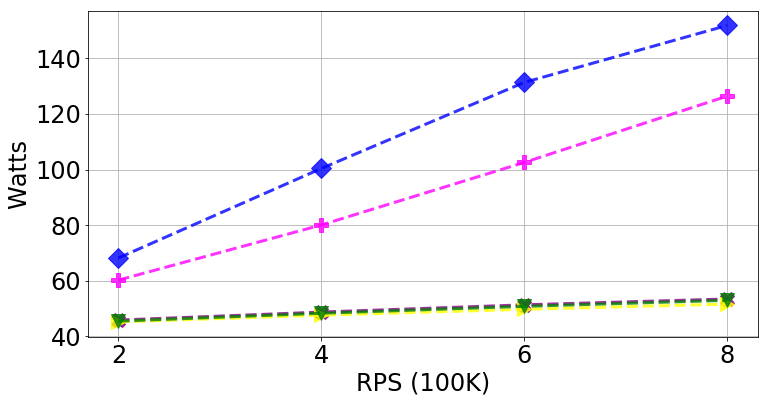
\includegraphics[width=\textwidth]{ebbrt_etc_pow_watts.png}
    \caption{}
    \label{fig:ebbrt_etc_pow:watts}
  \end{subfigure}
    \begin{subfigure}[b]{0.5\textwidth}
    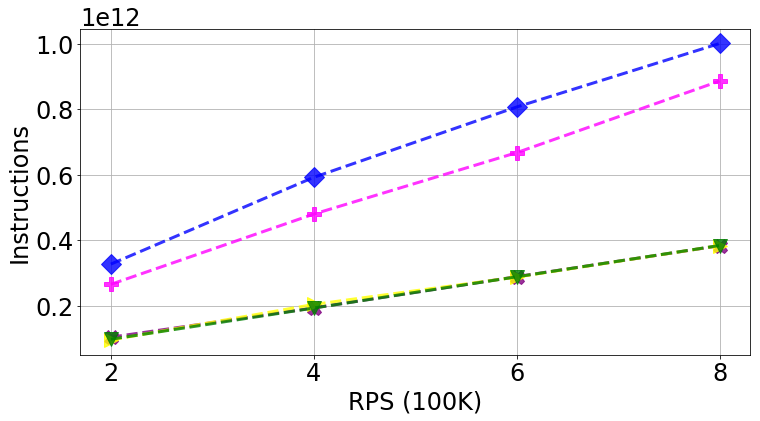
\includegraphics[width=\textwidth]{ebbrt_etc_pow_ins.png}
    \label{fig:ebbrt_etc_pow:ins}
  \end{subfigure}
  \begin{subfigure}[b]{0.5\textwidth}
    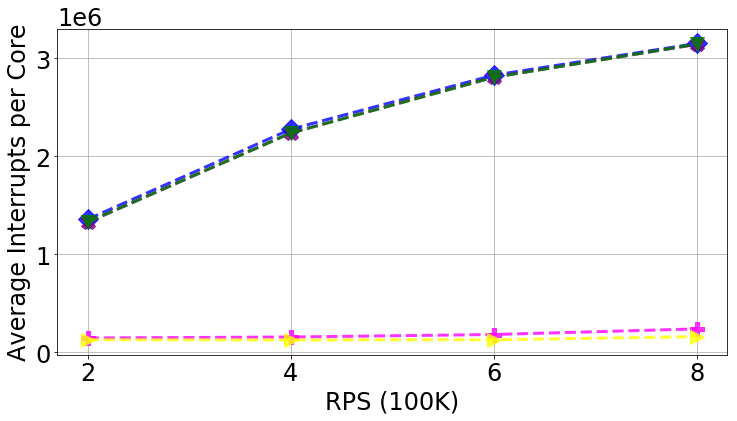
\includegraphics[width=\textwidth]{ebbrt_etc_pow_itr.png}
    \label{fig:ebbrt_etc_pow:itrs}
  \end{subfigure}
  \caption{EbbRT Memcached ETC workload in \textit{minimum} CPU frequency.}
  \label{fig:ebbrt_etc_pow:main}
\end{figure}

\begin{table}[h!]
\centering
\begin{tabular}{ |c|c|c|c|c| } 
 \hline
 RPS(100K) & 2 & 4 & 6 & 8 \\
 \hline
 Linux-ITR-16 & 1.1e+10 & 1.3e+10 & 1.4e+10 & 1.5e+10 \\
 EbbRT-ITR-16 & 5.4e+09 & 8.6e+09 & 1.1e+10 & 1.3e+10 \\
 \hline
\end{tabular}
\caption{Instructions/Watt comparison at different request loads for static interrupt delay at 16 microseconds.}
\label{tab:ins_per_watt2}
\end{table}

In contrast to Linux, Figure~\ref{fig:ebbrt_etc_pow:main} shows that changing processor frequency from maximum to minimum resulted in a 2X performance penalty in EbbRT. Unsurprisingly, this result also demonstrate that by running a specialized kernel for a particular network workload, the optimized dataplane path resulted in pushing the processing bottleneck onto the CPU. Therefore resulting in a 2X performance penalty when we artificially lowered the CPU's frequency. Past dataplane operating systems research demonstrated packet processing bottlenecks that exists in traditional systems software stack~\cite{ix, arrakis, ebbrt}, they were able to gain further performance advantages by optimizing the dataplane code path. In this example, we demonstrate that these systems will be more affected by CPU frequency tuning methods as their codebase is more optimized.

Even at the lowest CPU frequency, EbbRT was still able to achieve 25\% higher peak throughput than Linux. Further, it is able to satisfy the specified RPS rates at the lowest power usage overall. At a RPS rate of 800K, \textit{Linux-ITR-MAX} achieves a minimum power usage of 126 Watts while EbbRT was able to use 2.4X less power at 53 Watts. This result highlights the impact of processor tuning when used in conjunction with a more efficient systems software stack. 

The efficiency comparison numbers between EbbRT and Linux in Section~\ref{sec:ebbrt_max} shows that as EbbRT is more than 2X more efficient at using its instructions to do the same amount of work as Linux, therefore, changing the processor frequency had a much bigger impact on overall performance. This effect can also be seen in the relative reduction in power consumption between switching CPU frequency in Linux and EbbRT. In Linux, moving from a high frequency to a low frequency resulted in power savings between 4\%-40\% for a set of RPS loads under the SLA. For the same RPS loads in EbbRT, the power savings was between 56\%-200\%.

We also found that adding \textit{ITR-DELAY} and \textit{RAPL-MAX} to gain additional power savings in this setting had a minimal effect overall, with only additional power savings of 1\%-2\% on average. This phenomenon could be similar to results shown in Figure~\ref{fig:linux_etc_pow:watts} as the CPU is already operating at such a lower frequency that doing additional coalescing of receive packets and power limiting have a negligible overall effect on power consumption. While EbbRT uses 2.6X-3.1X fewer instructions compared to Linux in Figure~\ref{fig:ebbrt_etc_pow:ins}, Table~\ref{tab:ins_per_watt2} shows that an efficiency measure in terms of Instructions per Watt was only between 1.14X - 2X as the system is already operating in a minimal power setting. 

%-------------------------------------------------------------------------------

%Footnotes should be places after punctuation characters, without any
%spaces between said characters and footnotes, like so.%
%\footnote{Remember that USENIX format stopped using endnotes and is
%  now using regular footnotes.} And some embedded literal code may
%look as follows.

%-------------------------------------------------------------------------------
%\section{Floating Figures and Lists}
%\label{sec:figs}
%-------------------------------------------------------------------------------
\section{Related Work}
There have been past works that looked at energy proportional computing under strict SLA objectives when applied to in-memory key-value stores~\cite{10.1145/2678373.2665718, 10.1145/2806777.2806848}. They developed dynamic algorithms such as fine tuning CPU frequency via \textit{DVFS} or statically searching a large space and removing CPU cores in conjunction with \textit{RAPL} to lower overall power usage while maintaing SLA objectives. Our work takes a look at the same problem from a different angle by going directly at source of packet processing by delaying when packets actually get processed. The authors in ~\cite{10.1145/2806777.2806848} also looked at energy savings in the context of \textit{ix} a specialized library OS for Memcached, however, their measurements were taken in a virtualized environment while we used a baremetal library OS. In \cite{10.1145/2024723.2000103}, the authors proposed wholistic system optimization of CPUs, RAM and storage towards this energy proportional goal. Our work leads credence to their proposal by demonstrating a new aspect of NIC tuning that can be used. Overall, we do believe our work can co-exist with these other approaches as another layer on top of enabling better system efficiency while meeting SLA objectives in OLDI workloads.

There has been a large body of work in understanding complexity of device drivers~\cite{Kadav:2012:UMD:2150976.2150987} and various aspects of their reliability~\cite{Ball:2006:TSA:1217935.1217943, LeVasseur:2004:UDD:1251254.1251256, Ryzhyk:2009:DTD:1519065.1519095}, configuration~\cite{Renzelmann:2009:DMD:1855807.1855821, Ryzhyk:2014:UDD:2685048.2685101, Schupbach:2011:DLA:1950365.1950382}, and performance~\cite{Ganapathy:2008:DIM:1346281.1346303, Ryzhyk:2010:CAD:1851276.1851283}. The focus is mainly on device driver interface exposed to systems software, usually in order to provide a unified way to synthesize device drivers across different hardware and reduce code complexity while improving fault tolerance. While we do not address the inherent complexity in device drivers, our work shows the benefits if device driver interfaces are more accessibile towards application writers by exposing more hardware knobs that are easily tunable.

Similarly, there have been past projects to enable developers to make better use of NIC features by exposing NICs in a programmable way: FlexNIC~\cite{flexnic} enables dynamic modification of RSS rules to better load balance in Memcached, Affinity-Accept~\cite{affinityaccept} uses the Flow Director capability on IXGBE NICs in order to ensure TCP connections are always affinitized to the same core. Our work is inspired by these approaches in taking an advantage of another feature on the same Intel 82599 family of NICs and using it in a way that is more amenable towards an applications' energy goal.

There is a proliferation of new \textit{smart} hardware such as NICs~\cite{netronome, mellanoxsnic}, SSDs~\cite{biscuit}, and memory~\cite{dpu} to in order to bring computation closer to the data~\cite{neardataprocess, ndp1} and potentially improve overall application energy efficiency. Subsequently, these devices are expected to join the existing plethora of programmable accelerators~\cite{msrfpga, tpu} within a modern datacenter~\cite{silberstein1}. One potential problem posed by this diversity is the number of new knobs that are exposed to developers and how to better specialize towards their application. In this work, the benefits we show in tuning a single hardware register that exists on modern NICs stresses the importance in exposing more of these hardware knobs.

%-------------------------------------------------------------------------------
%\section*{Acknowledgments}
%-------------------------------------------------------------------------------
\section{Discussion and Future Work}
There are a few advantages and disadvantages to the \textit{ITR-Delay} mechanism. As it can only be set to a maximum of 1024 microseconds, it remains to be seen how its benefits fare in settings with SLA's in the milliseconds range. Further, it must also interact with retransmit timeout policies in the TCP/IP stack. Potentially if one delays the interrupt mechanism too long, it could cause redundant retransmissions and decrease overall throughput. \textit{ITR-Delay} can also be modified on a per receive queue basis, which are typically mapped to a distinct core. Potentially, if different workloads with different SLA objectives are consolidated on a single server node, it could be possible to customize interrupt receive delays on a per application basis while maintaing different SLAs across the diverse set of applications. This would result in even better additional power savings over methods such as \textit{RAPL} power limiting as it is a holistic approach that applies to the entire processor.

One aspect not covered in this work is the combination \textit{RAPL-MIN} and \textit{ITR-MAX} tuning, we did not explore this mainly due to the larger potential search space. For example, one approach would be to use first use \textit{ITR-MAX} to maximize interrupt delay and then apply \textit{RAPL-MIN} after while ensuring SLA objectives are still met, another would be the reverse of this process. The benefit of this can be seen in the figures above where \textit{RAPL-MIN} was able to lower power usage until a point where the application failed to launch, however, its 99\% tail latency was still greatly under the SLA. This presents an opportunity to then add \textit{ITR-MAX} to delay packet processing and enable additional power savings. Moreover, it is unknown if the best power savings actually derives from some intermediate combination of both methods. Given this, we are also interested in exploring the use of learning methods to bridge this large search space, the goal would be to develop a system module that can use application performance metrics combined with other metrics such as SLA in order to identify system configurations of CPU and the NIC that can optimize power savings as an objective.

Furthermore, there is an increasing need to readdress the complexity of modern NIC drivers~\ref{181902}, examining the Intel 82599 datasheet~\cite{82599} revealed over 5600 writable and read-only 32-bit registers and \textit{ITR-Delay} only represented one of them. Other than \textit{ITR-Delay} there are other hardware registered that have a direct on application processing of packets such as Receive Side Coalescing, as well as other tunable parameters in packet transmission. We are also interested in the impact that tuning these parameters have on a general purpose OS and a specialized OS. 

\section{Conclusion}
We present our work in exploiting the interrupt delay mechanism that exist on modern NICs to lower power usage in Memcached while maintaining SLA objectives for different low to medium level request rates. We compare and contrast this method with power limiting features under two different CPU frequency settings. One of the contributions of this work is demonstrating the advantages gained by catering static interrupt delay values to a application specific manner. The mechanism to delay packet processing can be tuned in a fine-grained manner at the microsecond scale, this enables greater control over request latencies. When applied in Linux, we were able to achieve peak power savings of 22\% over \textit{RAPL} power limiting. We also examined the impact of hardware tuning in a barmetal library OS specialized for Memcached. In this setting, we found that since a specialized library OS is able to take better advantage of CPU frequency, changing CPU frequency was able to save over 2X the power as compared to operating in highest CPU frequency while sacrificing 2X peak throughput. Further, we found that a baremetal library OS was able to achieve 2.5X higher peak throughput than Linux while using 3X lower power.

%-------------------------------------------------------------------------------
\bibliographystyle{plain}
\bibliography{bib}

%%%%%%%%%%%%%%%%%%%%%%%%%%%%%%%%%%%%%%%%%%%%%%%%%%%%%%%%%%%%%%%%%%%%%%%%%%%%%%%%
\end{document}
%%%%%%%%%%%%%%%%%%%%%%%%%%%%%%%%%%%%%%%%%%%%%%%%%%%%%%%%%%%%%%%%%%%%%%%%%%%%%%%%

%%  LocalWords:  endnotes includegraphics fread ptr nobj noindent
%%  LocalWords:  pdflatex acks
